\documentclass{article}[12pt]
\usepackage{graphicx}

\title{The AJIT multi-thread interrupt controllers}
\author{Madhav P. Desai}

\begin{document}
\maketitle

The AJIT interrupt controller for multiple-threads is shown below.
\begin{center}
  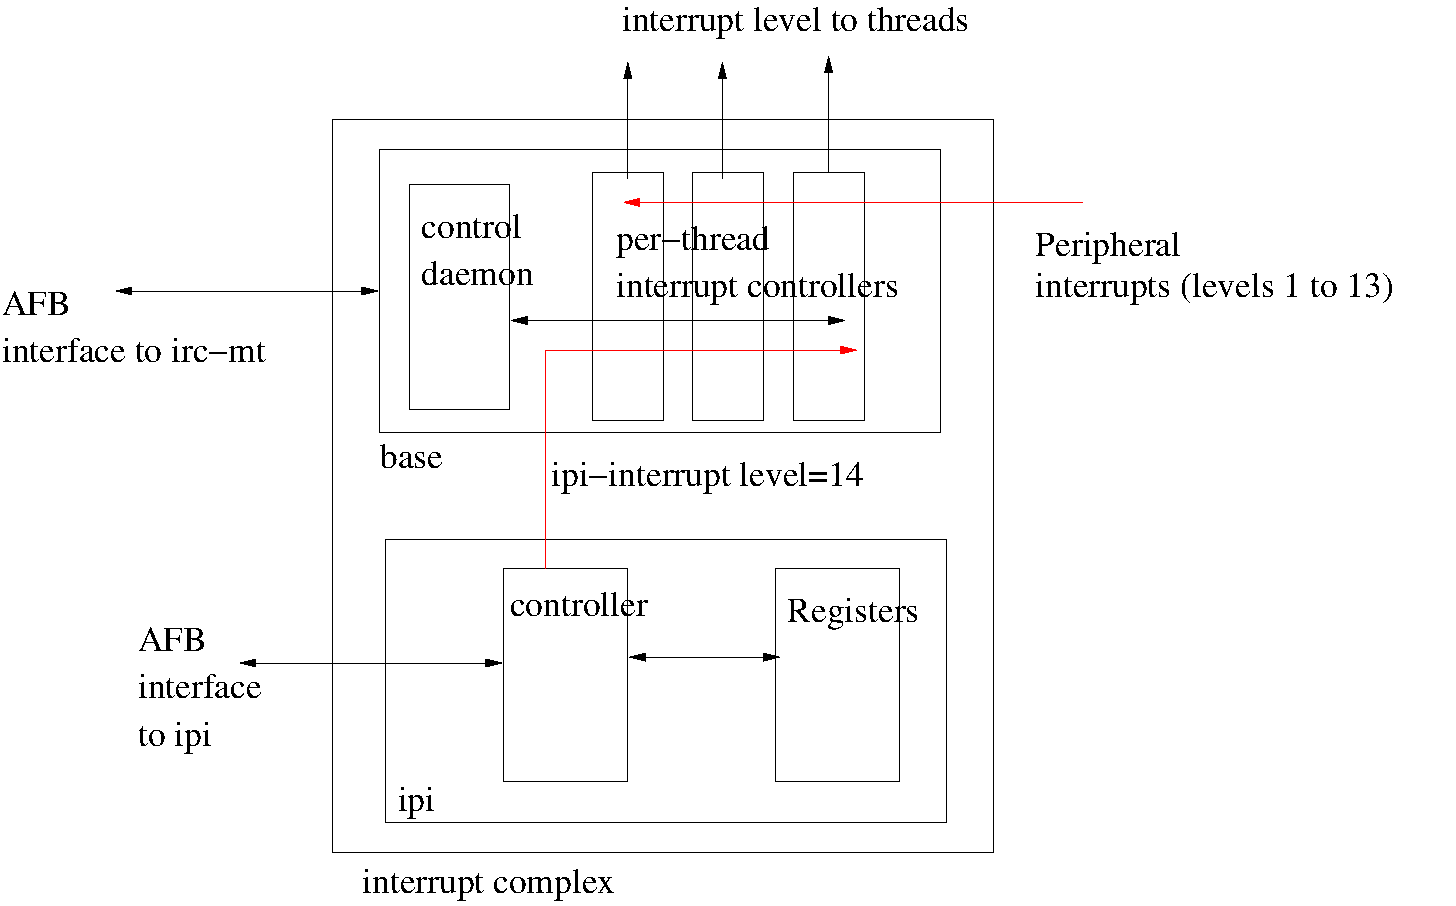
\includegraphics[width=12cm]{ajitInterrupt.pdf}
\end{center}
It consists of two components, a base multi-thread interrupt controller
and an inter-processor-interrupt controller.

As memory mapped I/O, the internal registers of the interrupt
controller are allocated 256 bytes (aligned to a 256 byte boundary).

\section{The base multi-thread interrupt controller}

Addresses from 0x0 to 0x7f are mapped to the base interrupt controller.

The base interrupt controller has up to 8 threads.
Each thread in the interrupt controller is associated with a CPU thread.
The maximum configuration corresponds to a four core processor with
each core having two threads.  CPU thread $(i,j)$ (where $0 \leq i \leq 3$, $0 \leq j \leq 1$)
is associated with interrupt controller thread $(2*i) + j$.

Each thread in the base interrupt controller observes primary interrupts from
the possible interrupt sources.  If appropriately programmed, the incoming interrupt
is forwarded to the corresponding CPU thread.  This control is exercised by
using the control register in each base interrupt controller  thread.   The
32-bit control register for CPU thread $(i,j)$ is accessible at an
address offset of $4 \times ((2*i) + j)$.

The control register contains the following fields:
\begin{verbatim}
------------------------------------------------------
bits        interpretation
------------------------------------------------------
[0]         enable-bit
              set by processor thread to enable
              interrupts to the thread.

[15:1]      interrupt-enable
              individual interrupt enables for 15
              interrupt levels. 

[30:16]     incoming-interrupt-values. 
               incoming interrupt values of interrupts
               from level 15 to 1
               
               writes to this part of the register are
               ignored.

[31]        in-interrupting-state.
               will be read as 1 if interrupt controller
               thread is in interrupting state.
               
\end{verbatim}

Note that
\begin{itemize}
\item In order to enable all interrupts to a particular thread 
we write the value 0xffff to the control register for that thread.
\item In order to disable all interrupts to a particular thread,
there are two ways.  The simplest is to set the control-register's
bit-0 to 0.  Alternatively, we can set bits [15:1] of the control
register to 0.
\end{itemize}

\section{The inter-processor-interrupt (IPI) controller}

Addresses from 0x80 to 0xff are mapped to the IPI controller.

The IPI controller is used for one processor thread to
trigger an interrupt on another (possibly the same) processor thread.

The IPI controller has the following registers
\begin{verbatim}
-----------------------------------------------------------------
offset-from-0x80          name  
-----------------------------------------------------------------
0                         ipi_interrupt-mask
                             bits [7:0] serve as 
                             a mask for IPI interrupt 
                             to destinations 7 down to 
                             0
4                          ipi-interrupt-value
                             bits [7:0] serve as 
                             a interrupt value for IPI 
                             interrupt to destinations 7 
                             down to 0

8 to 68                     ipi-data registers
                             Registers for keeping data
                             (arguments) which identify
                             the thread which has generated
                             interrupt etc.  USE OF THESE
                             BITS IS DETERMINED BY SOFTWARE.

76                          ipi-lock
                              These 4 bytes can be used as locks
                              by SOFTWARE.
-----------------------------------------------------------------
\end{verbatim}

To generate an IPI interrupt from thread $i$ to thread $j$, 
one must go through the following sequence at the source thread $i$:
\begin{enumerate}
\item Disable interrupts to thread $j$ using the base interrupt controller.
\item Acquire the IPI lock using the IPI lock register.
\item If the destination thread is $j$ and if the mask and values
bits with index $j$ are set (this means that the IPI to $j$ is already asserted), 
release the lock, enable interrupts to
thread $j$ and try again later.  Else
go to the next step.
\item Update message registers: for example keep the 
            source-core-id and the 
            physical address of a message buffer in memory, etc.
            in the message area for the destination thread.  
\item Set IPI interrupt-bit for the destination thread.
\item Set the IPI mask bit for the destination thread.
\item Release the IPI lock.
\item Enable interrupts to thread $j$ in the base interrupt controller.
\end{enumerate}

When the destination thread is interrupted with an IPI
interrupt, it must 
\begin{enumerate}
\item    Disable interrupts to the destination thread.
\item    Acquire the IPI lock for the destination thread.
\item    Reads message registers (determined by software).
\item    Write message registers (determined by software).
\item    Clear the IPI interrupt bit for the destination thread.
\item    Release the IPI lock.
\item    Enable interrupts to the destination thread.
\end{enumerate}

\end{document}


